\chapter{Teljesítménymérés, értékelés}

Ebben a fejezetben megvizsgálom az eszköz teljesítményét és azt, hogy hogyan skálázódik a funkcionalitás a modell elemszámának növekedésével. Ez azért fontos, mert  hiába van megoldásunk egy problémára, ha az a gyakorlatban az erőforrások korlátossága miatt nem képes időben eredményt adni. A két legfontosabb tényező az idő és a memóriafogyasztás. Megfelelő gyorsítótárak alkalmazásával az idő mértéke drasztikusan csökkenthető, viszont ez memóriába kerül. Ha a memória elfogy a szemét gyűjtő algoritmus agresszívabban próbálhatja összeszedni az elengedett objektumokat, ez szintén megnövelheti a végrehajtási időt, hiszen a rendszer szemétgyűjtéssel és nem pedig a működés elvégzésére használja az erőforrásokat.

A plugin VIATRA-t használ mégpedig inkrementális konfigurációval. Ez azt jelenti, hogy minták inicializációjuktól folyamatosan figyelik a modell változásait és módosítják a lekérdezések eredményhalmazát. Ez szintén memóriát vesz igényben viszont az elemek lekérdezése egy táblázat sorának kiolvasásának megfelelő komplexitással bír és nagyon gyors. Azt, hogy mennyire nő nagyra a VIATRA memória igénye leginkább a minták befolyásolják ezért különösen fontos, hogy ezek minél hatékonyabbak legyenek, mert nagy modell esetén nagyon nagy memória fogyasztást eredményezhetnek.

\section{Módszertan}

A teljesítmény mérés során az egyes transzformációk futási idejét és a VIATRA memória fogyasztását mértem. Magát a formális verifikációt  nem vizsgáltam, mert az főként az \uppaal\ teljesítményétől függ. Továbbá nem foglalkoztam különösebben az állapotgépek transzformációjának mérésével, mert ezt már vizsgálva volt a plugin korábbi változatában. A mérésekkel a kompozíciók skálázhatóságát vizsgáltam főként.

A méréseket a VisualVM\footnote{https://visualvm.github.io/} nevű java profilozó eszköz segítéségével végeztem. A futtatást mintavételezés segítségével profiloztam. Ez a módszer kevesebb beavatkozással jár a tényleges teljesítményt tekintve a futtatásba, viszont nem szolgáltat teljesen pontos képet, például a metódus hívások pontos számának megállapítására nem alkalmas. A másik lehetőséghez az instrumentális profilozás ami, nagyobb \emph{overhead}del jár viszont pontosabb képet adhat.

A mérések a következő specifikációk mellett lettek elvégezve:
\begin{center}
	\begin{tabular}{ l r }
MagicDraw verzió & 19 \\
Heap méret & 10G \\
Operációs rendszer & Windows 10\\
CPU & Intel i5-10600K\\
	\end{tabular}
\end{center}

\section{Végrehajtási idő változása az elemek számával}

Az első mérés során azt vizsgáltam, hogy a partok és az őket tipizáló blokkok számának növelésével milyen mértékben növekszik a végrehajtási idő. Ehhez készítettem egy pár állapotból és címkézetlen átmenetekből álló állapotgép definíciót és ezt másolgatva növeltem a állapotgép definíciók és az velük tipizált partok mennyiségét (\ref{fig:part_mes1} ábra).

\begin{figure}[!ht]
	\centering
	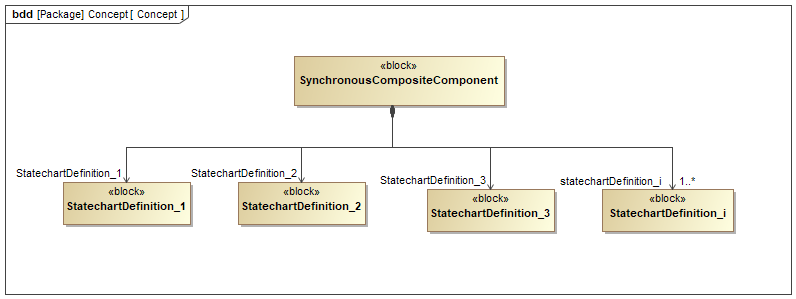
\includegraphics[width=12cm, keepaspectratio]{figures/evaluation/part_mes.png}
	\caption{Méréshez használt modell}
	\label{fig:part_mes1}
\end{figure}

A méréseket tíz, húsz, harminc, negyven és ötven part méretek mellett végeztem el. Az eredmények kezdetben elég lesújtóak voltak, nem árulkodtak túl jó skálázhatóságról és a végrehajtási idők is nagyon magasak voltak. A mérési eredmények \aref{fig:mes1} ábrán láthatók.


\begin{figure}[!ht]
	\centering
	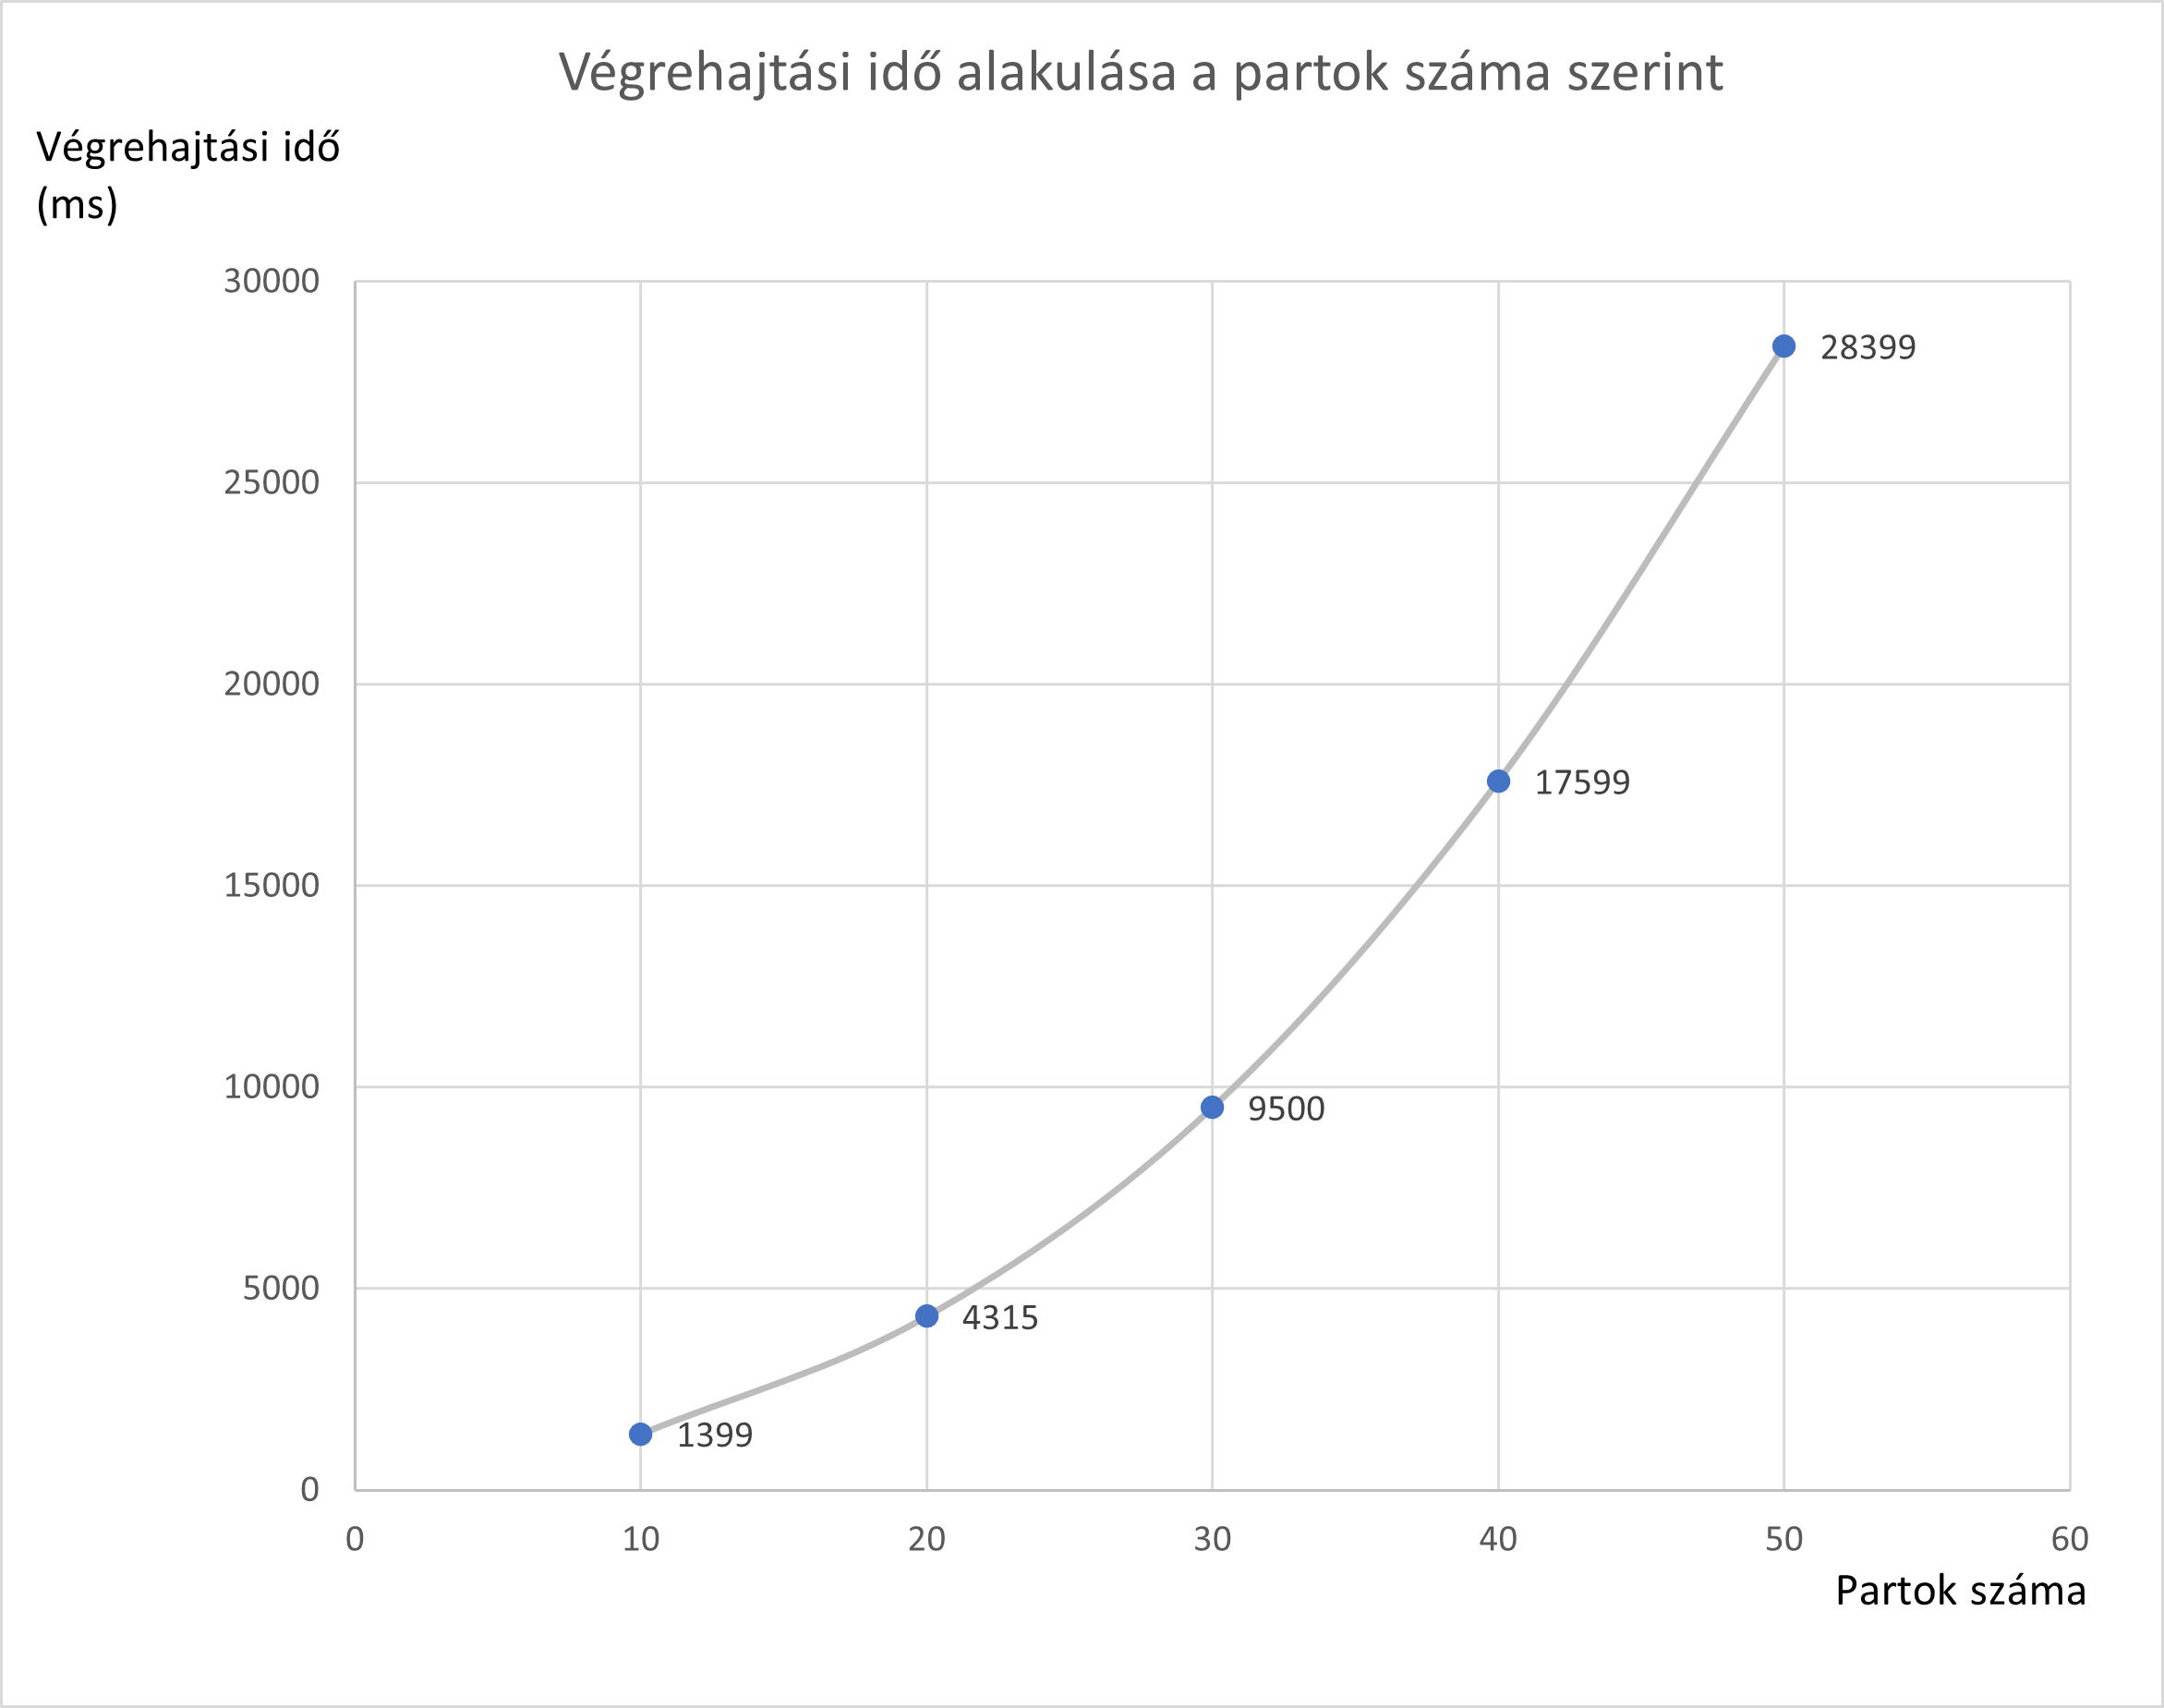
\includegraphics[width=12cm, keepaspectratio]{figures/evaluation/mes-1.png}
	\caption{Első mérés eredményei}
	\label{fig:mes1}
\end{figure}

Behatósabban vizsgálva a méréseket kiderül, hogy a legtöbb időt nem magának a transzformációnak a végrehajtása hanem az elemek visszakereshetőségét biztosító \emph{trace} modellek létrehozása emészti fel \footnote{Ez a visualvm-ben a modell session lázárásaként jelenik meg, ekkor véglegesülnek a modellen végzett módosítások}. Ez jelen esetben minden parthoz 18 \emph{property} létrehozását jelenti a modellben. A legnagyobb modell esetében 900 modell \emph{property}t kell létrehozni. Ennek fényében úgy tűnik, hogy a \emph{trace} modell ilyen módon történő tárolása nem a legjobb mérnöki megoldás.



Mivel a lassulás a MagicDraw működéséből keletkezik megpróbáltam másféle modell elemeket létrehozni \emph{property}k helyett remélve így kisebb lesz az elemek létrehozásának a működésre gyakorolt hatása. \emph{Property}k helyett az EMF modellt szimbolizáló linkeket \emph{Class} példányokra cseréltem és újból elvégeztem a mérést. Az eredmények jelentős teljesítmény javulást mutatnak melyet az alábbi táblázat és \aref{fig:mes-2} ábra mutat.\\

\begin{center}
	\begin{tabular}{ lccccccccc }
		Partok száma & 10 & 20 & 30 & 40 & 50 & 100 & 200 & 500 & 1000 \\
		\hline
		Teljes futási idő & 699 & 798 & 1098 & 1599 & 1899 & 3300 & 2400 & 7000 & 12799 \\
		Transzformáció & 100 & 99 & 98 & 199 & 200 & 301 & 700 & 2000 & 4240\\
	\end{tabular}
\end{center}

 A diagramon a függőleges tengely logaritmikus. A diagramról megállapítható, hogy a végrehajtási idő lineárisan változik a \emph{part}ok darabszámának növekedésével. Ugyanakkor az is látszik, hogy ugyan a korábbi implementációkhoz képest sokkal kevésbé jelentős a \emph{trace} modell létrehozásának az ideje, de az elemszám növekedésével rosszabban skálázódik, mint maga a transzformáció, így kellően nagy modelleken ezzel a megoldással is dominálni fog.

\begin{figure}[!ht]
	\centering
	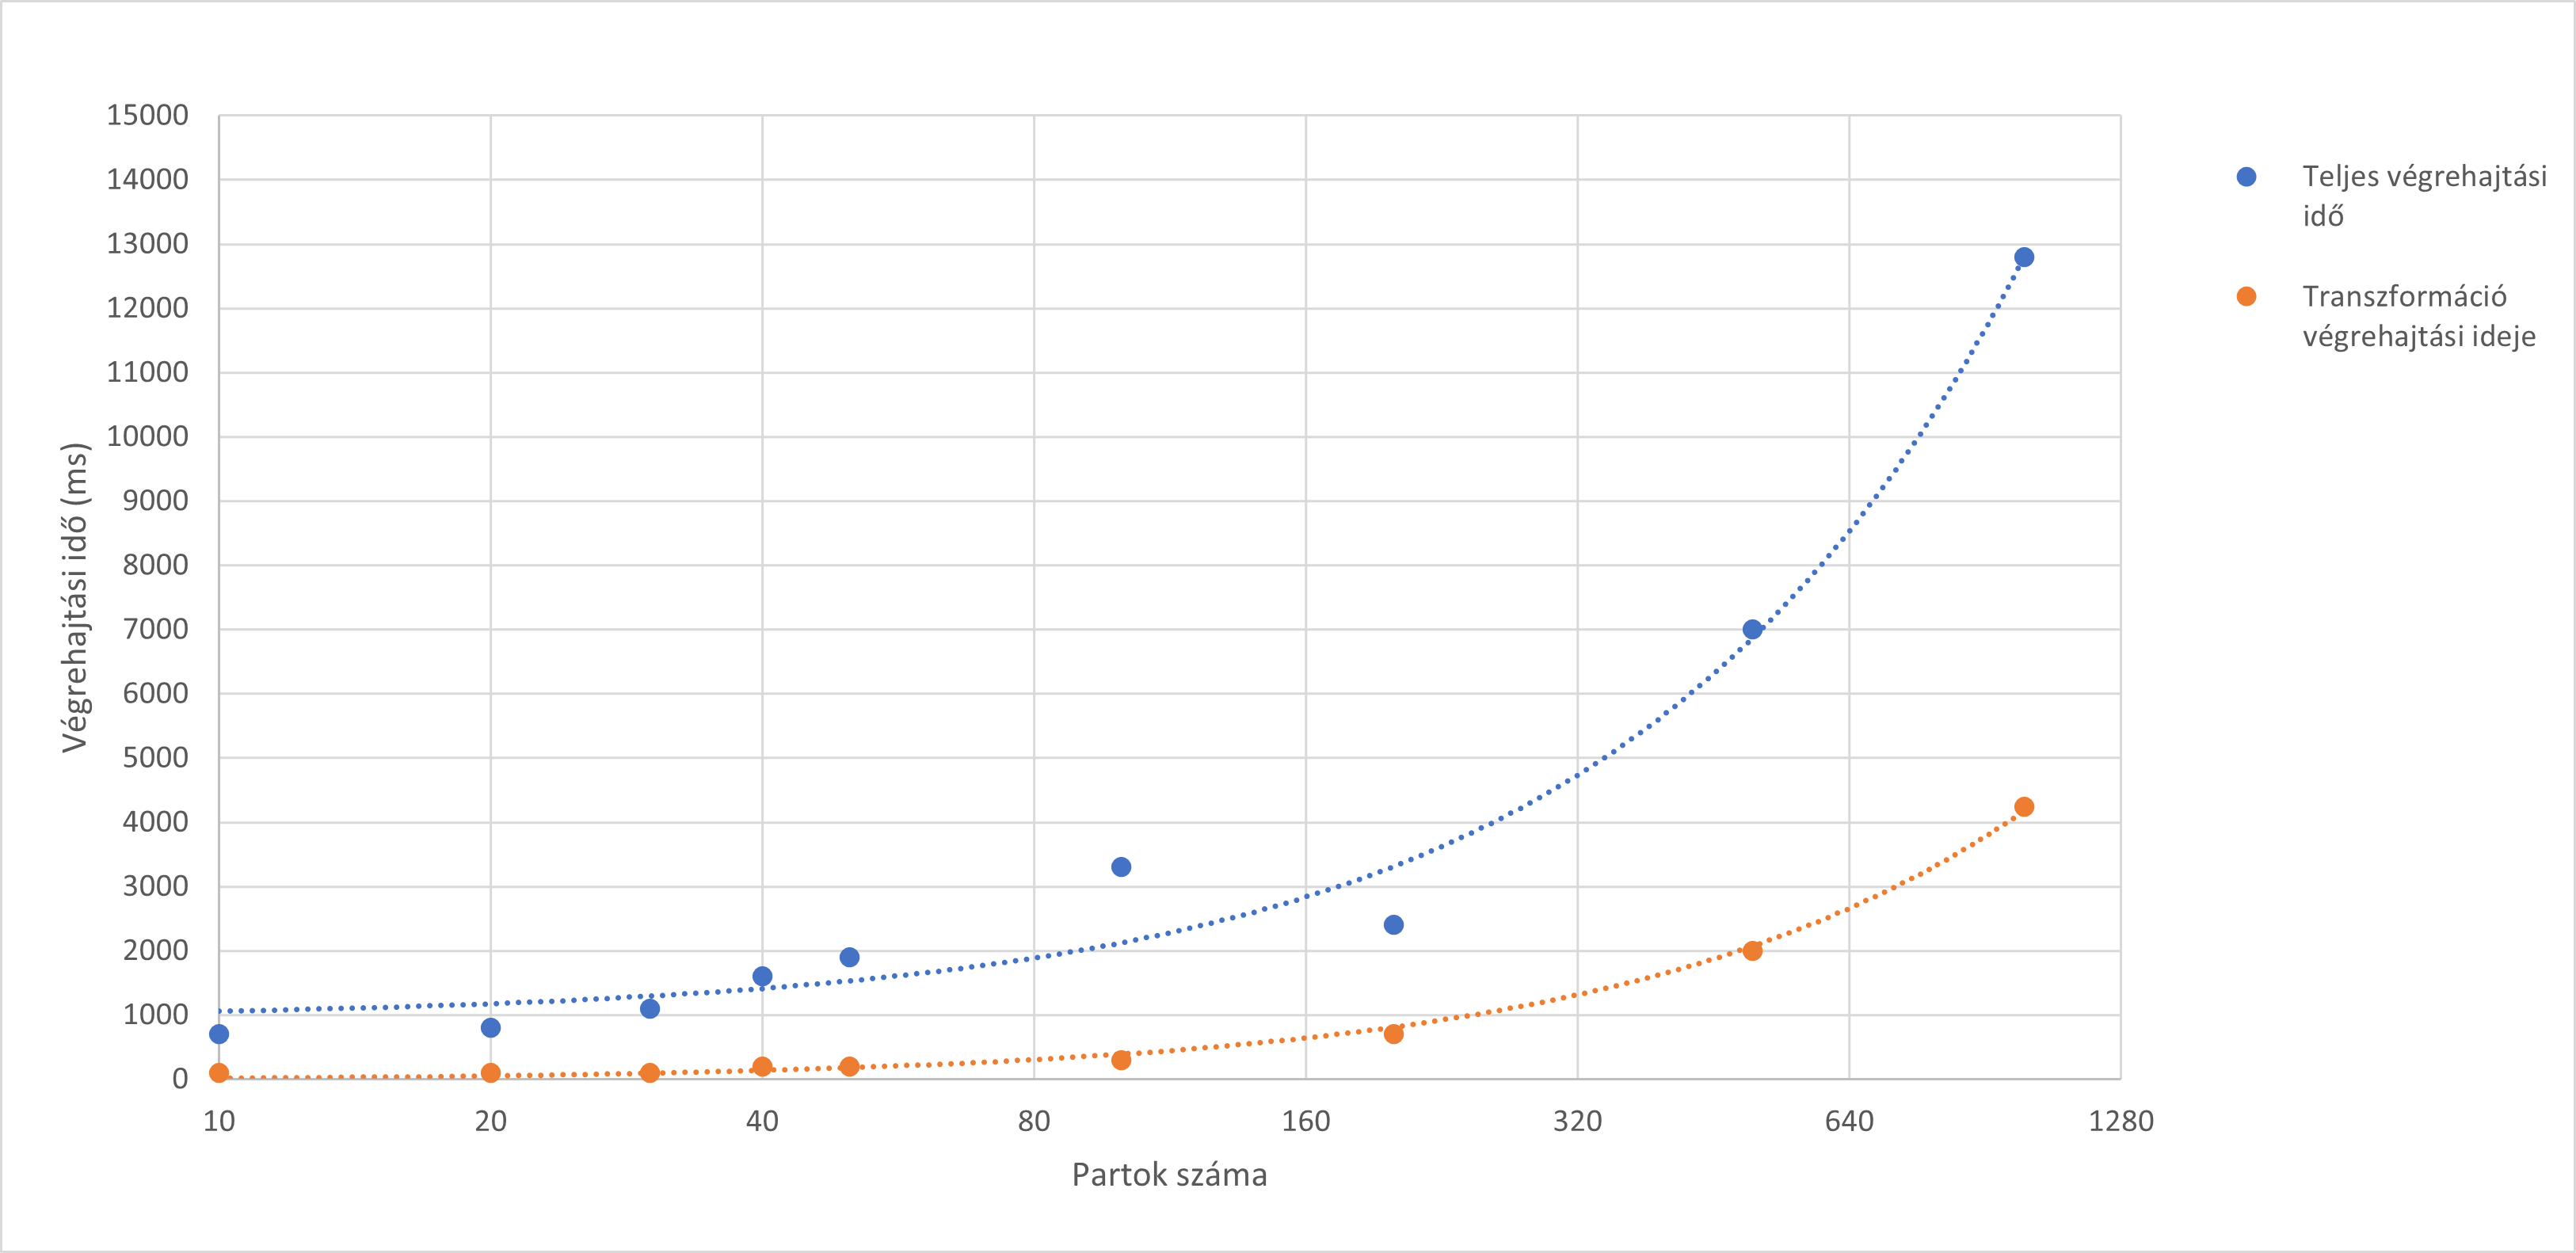
\includegraphics[width=12cm, keepaspectratio]{figures/evaluation/mes-2.png}
	\caption{Végrehajtási idők \emph{Class}ok használatával}
	\label{fig:mes-2}
\end{figure}

\paragraph{Értékelés:} A mérések alapján az derül ki, hogy a \emph{trace} modellek az ismertetett módon történő tárolása nagyon erős mértékben rontja az eszköz transzformációs teljesítményét. Egy lehetséges alternatíva egy EMF alapú modell létrehozása lehetne, amit szöveges formában le lehetne tárolni egy modell elemben - hasonlóan az Gamma állapottérképek XMI formában történő tárolásához - és ezzel összekapcsolni a két modellt.

\section{Memória igény változása az elemek számával}

A plugin projekt betöltésekor inicializálja a VIATRA mintákat, melyeket a transzformáció használ. Ez jelentősen meg tudja gyorsítani magát a transzformációt és azokat a validációs szabályokat melyek használják, viszont a találatok tárolási tárigényes. Ráadásul első induláskor be kell indexelni a modellt, ami megnöveli a projektek betöltésének idejét is. Mivel a tesztek során ebből fakadó problémát nem észleltem az indexelési időt nem vizsgáltam.

A memória használat méréséhez generált modelleket használtam. Minden állapotgép "n" hosszú állapot láncokból állt plusz egy kezdő állapotból. Az állapotok további "n" hosszú állapotláncokat tartalmaznak, melyek ismét tartalmaznak "n" hosszú láncokat és így tovább. Minden állapotátmeneten egy \emph{true} őrfeltétel van (példa: \ref{fig:generated} ábra).
\begin{figure}[!ht]
	\centering
	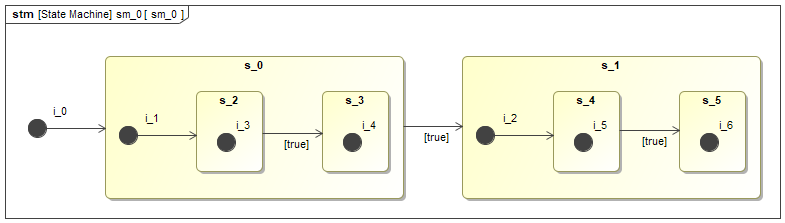
\includegraphics[width=12cm, keepaspectratio]{figures/evaluation/generated.png}
	\caption{Generált állapotgép 12+1 elemmel és 2 hosszú láncokkal}
	\label{fig:generated}
\end{figure}
\newpage
Minden végzett méréshez egy azonosítót rendeltem \emph{m-n-k} alakban. A mérések azonosítójában szereplő számpár (n és k) a generált modell paramétereire utalnak. Az első szám a csomópontok száma (állapotok és kezdőállapotok) a második szám pedig a láncok hosszát jelenti. Fontos, hogy az állapotok  egymásba ágyazottságának a mértéke is növelheti a VIATRA által karbantartott táblák számát. Az alábbi minta például tranzitív lezárt segítségével adja vissza egy állapotgép régióinak számát.
\begin{lstlisting}
pattern RegionsInStatechart(stmt: StateMachine, region: Region){
   find MainRegions(stmt, region);
} or {
   find MainRegions(stmt, outerRegion);
   find InnerRegion+(outerRegion, region);
}
\end{lstlisting}
 A beágyazottság mértéke az elemszám és a láncok hosszának hányadosa.\\

A mért értékeket a  következő táblázat tartalmazza. A MagicDraw által használt memória méretét az indexelés előtt mértem.\\

\hspace*{-1cm}
\begin{tabular}{l|ccccc}
azonosító: & m-1000-10 & m-5000-10 & m-10000-10 & m-20000-10 & m-100000-10 \\
\hline
kezdő állapotok: & 111 & 1111 & 1111 & 8891  & 11111 \\
állapotok:  & 890 & 3890 & 8890 & 11110 & 88890 \\
régiók: & 111 & 1111 & 1111 & 8891 & 88890\\
átmenetek: & 890 & 3890 & 8890 & 11110 & 88890\\
\hline
VIATRA (MB) & 19,8 & 26,7 & 36,3 & 62,2 & 377,4\\
MagicDraw (MB) & 264 & 267 & 368 & 657 & 2144,5 \\
\end{tabular}
\hspace*{-1cm}\\
\\
 
 \Aref{fig:mem1} ábrán az egész heap látható. Ebből az látszik, hogy ugyan a legnagyobb modellen már egészen nagy helyet foglal a VIATRA. A beágyazottság viszont ezen a modellen már egész magas, öt mély. A gyakorlatban egy állapotgépen az állapotok túlzott egymásba ágyazottsága nem annyira valószínű, hiszen ezzel együtt a komplexitása is nagyon magas lesz a modellnek ami általában kerülendő.
 \begin{figure}[!ht]
 	\centering
 	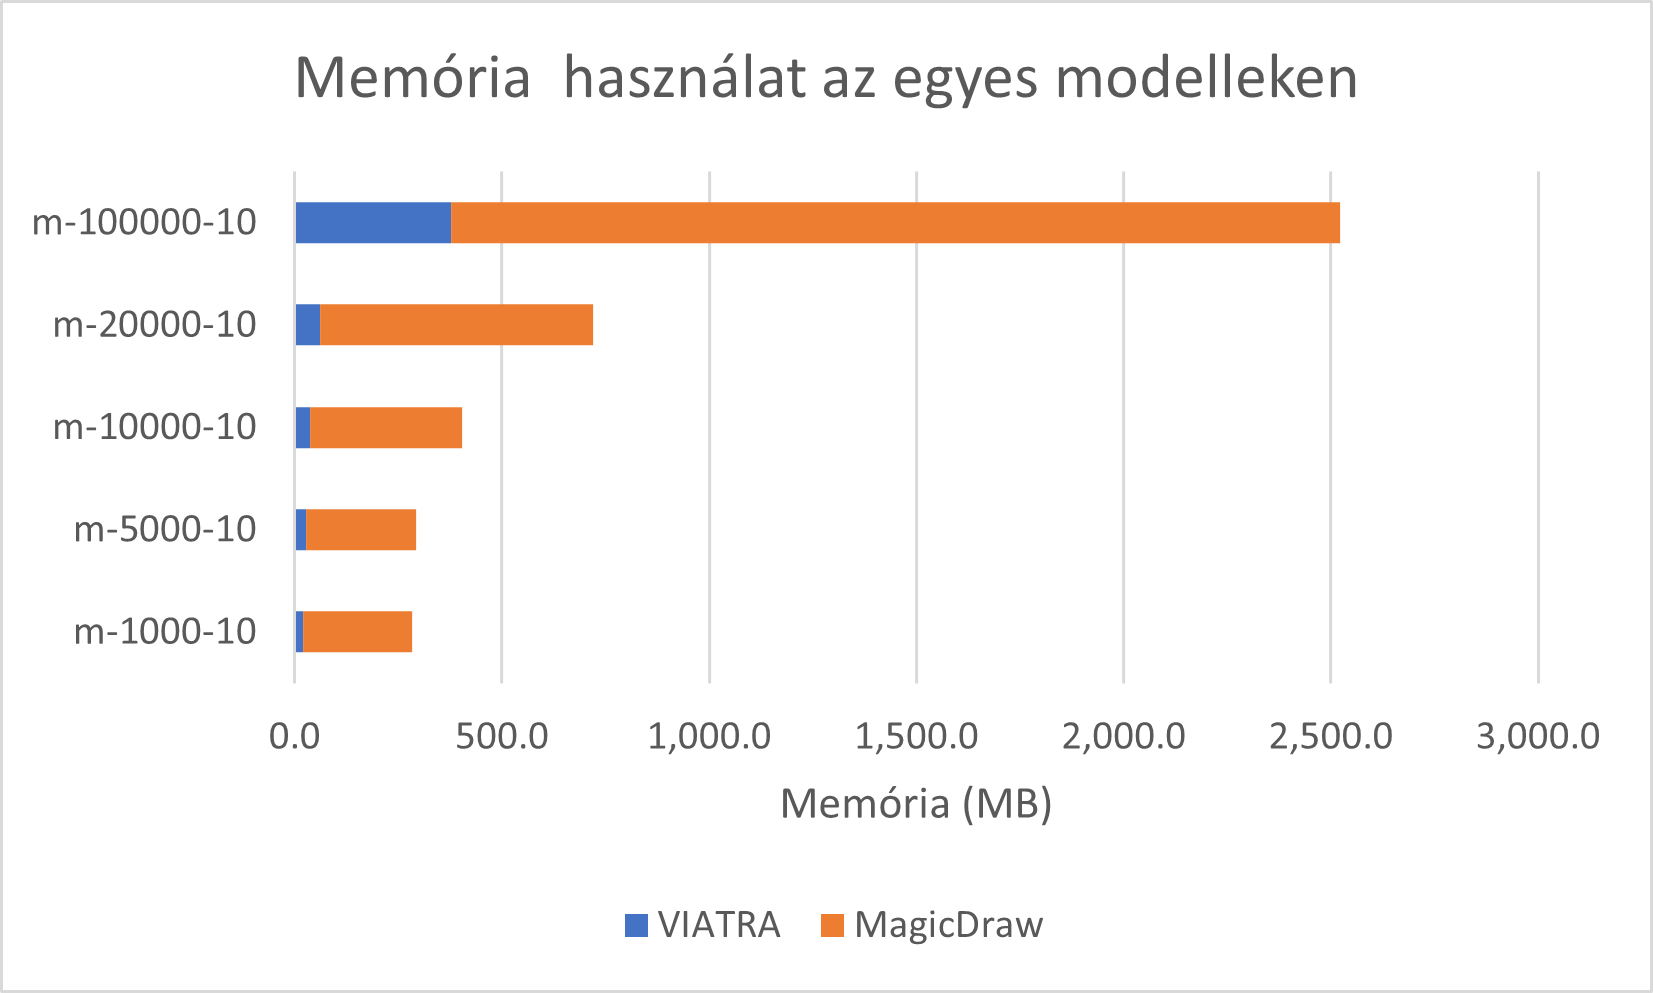
\includegraphics[width=12cm, keepaspectratio]{figures/evaluation/mem1.png}
 	\caption{Heap mérete és eloszlása}
 	\label{fig:mem1}
 \end{figure}
\newpage
A meómria használat eloszlását picit részletesebben nézzük (\ref{fig:mem2} ábra) akkor azt látjuk, hogy a legnagyobb és a legkisebb modell között a VIATRA nagyobb arányban használja a memóriát majdnem kétszer annyit.
 \begin{figure}[!ht]
	\centering
	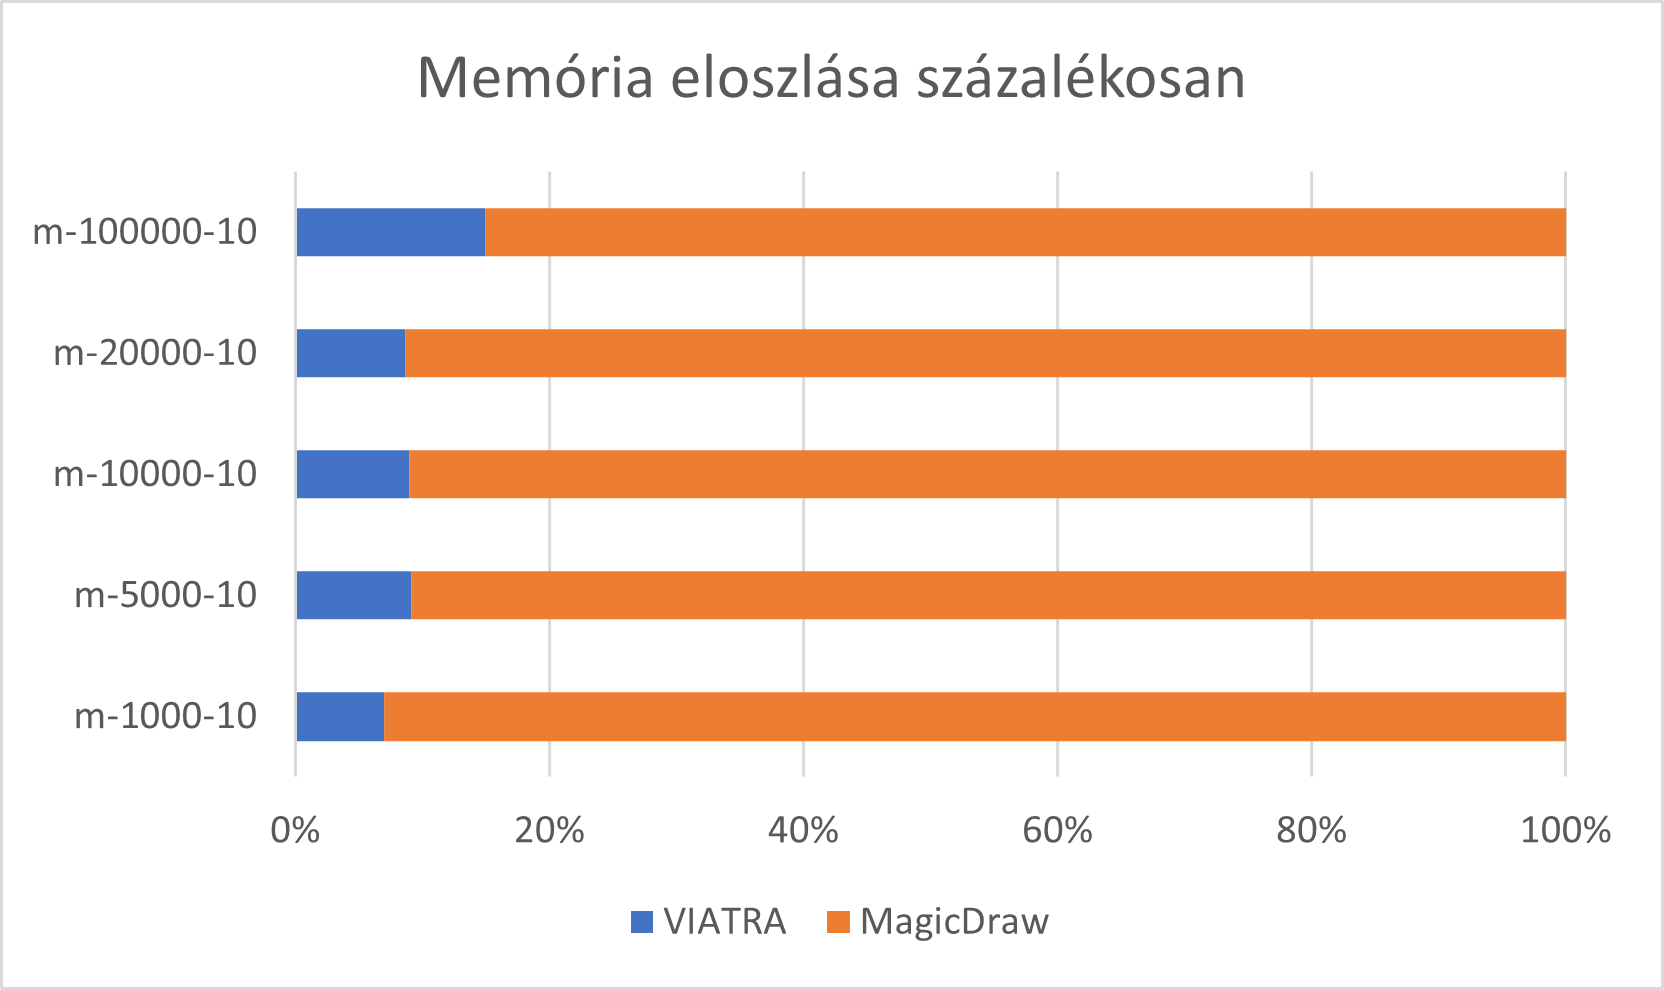
\includegraphics[width=12cm, keepaspectratio]{figures/evaluation/mem2.png}
	\caption{Heap méretének százalékos eloszlása}
	\label{fig:mem2}
\end{figure}
Ennek két fő oka lehet. Az egyik, hogy a mérések során a MagicDraw teljes memóriahasználatát néztem a mibe beletartoznak az importált modellek is mint például a SysML projekt és a Gamma profil is. Ez szám ugyan állandó, de a kisebb méreteken dominálhat, míg a nagyobb méreteken már az a generált állapogép mérete lesz a meghatározó. A másik a már említett egymásba ágyazottság növekedésének mértéke.

\paragraph{Értékelés:} a mérések során nem tapasztaltam kiugró mértékű teljesítmény csökkenést, ami azt jelenti, hogy a vizsgált minták között nem volt olyan, ami nem lett elég jól megírva. Ugyanakkor a közel 18\%-os eredmény a legnagyobb modellen indokolttá teheti, hogy nagy modelleken a VIATRA ne fusson folyamatosan, hanem ez kikapcsolható legyen.





